\chapter{Reinforcement Learning Basics}
\label{ch:rl}

\chapterguide%
  {Probability, expected value, optimization, and the idea of sequential decisions.}
  {describe a problem as states, actions and rewards; balance exploring with exploiting; compute a discounted return; run Q-learning updates by hand; read a policy from a Q-table; and evaluate a greedy policy separately from training.}

Nobody hands a puppy a table of correct actions. It sits, and it gets a treat. It chews a shoe, and it does not. Reinforcement learning (RL) learns the same way: there is no answer column at all, only a score that arrives after the learner acts, sometimes much later. Because actions change what happens next, the goal is not one good move but a good long run.

\begin{coursechoice}
Lab~6 implements tabular RL. Neural function approximation for deep RL lies beyond this course.
\end{coursechoice}

\section{The agent-environment loop}

At time $t$:

\begin{utpsteps}
  \item The agent observes a state $s_t$.
  \item It chooses an action $a_t$.
  \item The environment returns a reward $r_{t+1}$ and a new state $s_{t+1}$.
  \item The agent updates what it believes about the action.
\end{utpsteps}

\begin{utpfig}[The agent-environment loop]{The agent-environment loop. The agent chooses an action; the environment changes state and returns a reward and the new state.}{fig:agent-environment}
\begin{tikzpicture}[
  node distance=3.5cm,
  box/.style={draw=UTPBlue,fill=UTPPaleBlue,rounded corners=2mm,minimum width=3cm,minimum height=1.2cm,align=center,font=\bfseries\color{UTPNavy}},
  arr/.style={-{Stealth[length=2.4mm]},thick,draw=UTPTeal}
]
\node[box] (agent) {Agent\\chooses an action};
\node[box,right=of agent] (env) {Environment\\changes state};
\draw[arr] (agent.north east) to[bend left=18] node[above,font=\small]{action $a_t$} (env.north west);
\draw[arr] (env.south west) to[bend left=18] node[below,font=\small]{state $s_{t+1}$, reward $r_{t+1}$} (agent.south east);
\end{tikzpicture}
\end{utpfig}

\begin{workedexample}
A warehouse robot tracks location and battery, chooses movement or charging, and balances time and collision costs against delivery rewards.
\end{workedexample}

\section{A simpler case: which food stall?}

\begin{analogy}
Three stalls near campus serve lunch. You have a favorite. Tomorrow you could go back to it, or try the one you have never tried, which might be better or might waste a lunch. Every choice both feeds you and teaches you, and you cannot do both fully at once.
\end{analogy}

This creates the central RL problem:

\begin{description}[leftmargin=1.35in,style=nextline]
  \item[Exploration] Try uncertain actions to learn more about them.
  \item[Exploitation] Choose the action currently believed to be best.
\end{description}

An $\varepsilon$-greedy strategy explores with probability $\varepsilon$ and otherwise exploits.

\begin{workedexample}
Three stalls give a good meal with hidden chances 0.2, 0.5 and 0.8. A student keeps a running average for each stall, and eats 1,000 lunches. Averaged over 500 students:

\medskip
\centering\small
\begin{tabular}{@{}lcccc@{}}
\toprule
\rowcolor{UTPPaleBlue!92}
\utpth{Strategy} & \utpth{Visits: stall 1} & \utpth{Stall 2} & \utpth{Stall 3} & \utpth{Good meals per lunch} \\
\midrule
$\varepsilon=0$: never explore & 1000 & 0 & 0 & 0.199 \\
$\varepsilon=0.1$: explore one lunch in ten & 54 & 57 & 889 & 0.750 \\
$\varepsilon=0.5$: explore half the time & 168 & 170 & 662 & 0.648 \\
\bottomrule
\end{tabular}
\par\raggedright
\medskip
With no exploration, the student goes to the first stall, finds it acceptable, and never learns that a better one exists. Too much exploration keeps paying to learn something already known. The best possible rate is 0.8, and a little exploration gets close.
\end{workedexample}

\section{Markov decision processes}

A classical RL problem is often written as a Markov decision process (MDP) with:

\begin{itemize}
  \item a set of states $\mathcal{S}$;
  \item a set of actions $\mathcal{A}$;
  \item transition probabilities $P(s'\given s,a)$;
  \item a reward rule;
  \item a discount factor $\gamma\in[0,1)$.
\end{itemize}

Under the Markov assumption, the current state and action contain the information needed for the next-state distribution.

\section{Return and discounting}

A reward now is worth more than the same reward later, and the \term{discount factor} $\gamma$ says by how much. The \term{return} from time $t$ is the discounted sum of future rewards:
\[
  G_t=r_{t+1}+\gamma r_{t+2}+\gamma^2r_{t+3}+\cdots.
\]

\begin{workedexample}
Future rewards are $5,4,3$. With $\gamma=0.9$, $G_t=5+0.9(4)+0.81(3)=11.03$. With $\gamma=0.5$ the return is 7.75. With $\gamma=0$ only the next reward counts, giving 5, and with $\gamma=1$ all count equally, giving 12.
\end{workedexample}

\section{Policies and value functions}

A \term{policy} $\pi(a\given s)$ describes how the agent chooses actions in each state.

The state-value function is
\[
  V^{\pi}(s)=\mathbb{E}_{\pi}[G_t\given s_t=s],
\]
the expected return from state $s$ while following policy $\pi$.

The action-value function is
\[
  Q^{\pi}(s,a)=\mathbb{E}_{\pi}[G_t\given s_t=s,a_t=a],
\]
the expected return from taking action $a$ in state $s$ and then following $\pi$.

\begin{intuition}
$V(s)$ asks, ``How good is this situation?'' $Q(s,a)$ asks, ``How good is this particular move from this situation?''
\end{intuition}

\section{The Bellman idea}

A long-term value can be broken into two parts:

\[
\text{value now}=\text{reward next}+\text{discounted value later}.
\]

For an optimal action-value function,
\[
Q^*(s,a)=\mathbb{E}\left[r_{t+1}+\gamma\max_{a'}Q^*(s_{t+1},a')\mid s_t=s,a_t=a\right].
\]
This recursive relationship is the basis of Q-learning.

\section{Tabular Q-learning}

When the state and action spaces are small, store one Q-value for every state-action pair in a table. After observing the transition $(s_t,a_t,r_{t+1},s_{t+1})$, update
\[
Q(s_t,a_t)\leftarrow Q(s_t,a_t)+\alpha\left[r_{t+1}+\gamma\max_{a'}Q(s_{t+1},a')-Q(s_t,a_t)\right].
\]
The quantity in brackets is the \term{temporal-difference error}: what just happened, plus the best you now expect from where you landed, minus what you believed. The estimate moves a fraction $\alpha$ of the way towards that new evidence.

\begin{utpsteps}
  \item Initialize the Q-table, often with zeros.
  \item Observe the current state.
  \item Choose an action using an exploration strategy such as $\varepsilon$-greedy.
  \item Perform the action and observe reward and next state.
  \item Update the chosen Q-table entry.
  \item Repeat over many episodes, gradually reducing exploration when appropriate.
\end{utpsteps}

\begin{workedexample}
\textbf{One update.} With $Q(s,a)=2$, $r=1$, $\gamma=0.9$, next-state maximum 4 and $\alpha=0.5$: the backup is $1+0.9\times4=4.6$, the TD error is $2.6$, and $Q(s,a)\leftarrow2+0.5(2.6)=3.3$.

\textbf{Value walks backwards.} A corridor of cells 0, 1, 2, then a goal worth $+1$. The agent always walks right, with $\alpha=0.5$ and $\gamma=0.9$, and all Q-values start at zero. Here is $Q(\text{cell},\text{right})$ after each trip:

\medskip
\centering\small
\begin{tabular}{@{}cccc@{}}
\toprule
\rowcolor{UTPPaleBlue!92}
\utpth{Episode} & \utpth{Cell 0} & \utpth{Cell 1} & \utpth{Cell 2} \\
\midrule
1 & 0.0000 & 0.0000 & 0.5000 \\
2 & 0.0000 & 0.2250 & 0.7500 \\
3 & 0.1013 & 0.4500 & 0.8750 \\
4 & 0.2531 & 0.6188 & 0.9375 \\
\bottomrule
\end{tabular}
\par\raggedright
\medskip
In episode 1 only the cell beside the goal learns anything. In episode 2 its value reaches the next cell back: $0.5\times(0+0.9\times0.5)=0.225$. News of the reward spreads backward, one cell per trip. That is why tabular RL needs so many episodes.
\end{workedexample}

\section{One Q-learning update, drawn}

The diagram separates a Q-update into its current estimate, backup value, and step size.

\begin{utpfig}[One Q-learning update]{One Q-learning update. The new estimate moves the old one a step of size $\alpha$ towards the backup value: what actually happened nudges what you believed.}{fig:q-update}
\begin{tikzpicture}[
  node distance=0.42cm and 0.8cm,
  bx/.style={draw=UTPBlue,fill=UTPPaleBlue,rounded corners=1.5mm,minimum width=2.5cm,minimum height=0.85cm,align=center,font=\scriptsize\bfseries\color{UTPNavy}},
  gd/.style={draw=UTPGreen,fill=UTPPaleTeal,rounded corners=1.5mm,minimum width=2.5cm,minimum height=0.85cm,align=center,font=\scriptsize\bfseries\color{UTPNavy}},
  op/.style={draw=UTPOrange,fill=UTPPaleOrange,rounded corners=1.5mm,minimum width=3.6cm,minimum height=0.82cm,align=center,font=\scriptsize\bfseries\color{UTPNavy}},
  arr/.style={-{Stealth[length=2mm]},thick,draw=UTPTeal}
]
\node[bx] (old) at (-2.35,1.55) {Old estimate\\$Q(s,a)$};
\node[gd] (backup) at (2.35,1.55) {Backup value\\$r+\gamma\max_{a'}Q(s',a')$};
\node[op] (update) at (0,0.30)
  {Move a fraction $\alpha$ toward the backup value\\$Q+\alpha(\text{backup}-Q)$};
\node[bx] (new) at (0,-1.05) {New estimate\\$Q(s,a)$};
\draw[arr] (old.south)--(update.north west);
\draw[arr] (backup.south)--(update.north east);
\draw[arr] (update.south)--(new.north);
\node[font=\scriptsize\itshape\color{UTPMuted},below=0.25cm of new,align=center]
  {what actually happened\\nudges what you believed};
\end{tikzpicture}
\end{utpfig}

\section{Lab~6's grid, solved}

Lab~6 trains on a $4\times4$ grid: start top-left, goal bottom-right worth $+1$, a trap at row 1, column 3 worth $-1$, and $-0.04$ per step, with $\gamma=0.95$. The shortest route takes six moves, so its plain return is $5\times(-0.04)+1=0.80$, and its discounted return from the start is 0.593.

We can compute the best possible value of every cell directly, by repeating the Bellman idea until nothing changes. \figref{fig:grid-values} shows the result. Lab~6's table, trained only from its own trial and error, reaches these same values to three decimals.

\begin{utpfig}[The best value of every cell]{Best possible values on Lab~6's grid, with the policy the lab's agent learns. Values rise towards the goal. The cell above the trap is worth only 0.666, less than its left neighbor's 0.743, because it has to step back left to get round the trap.}{fig:grid-values}
\begin{tikzpicture}[x=1.15cm,y=1.15cm,
  gv/.style={draw=UTPBlue!55,minimum size=1.15cm,inner sep=0pt,align=center,font=\scriptsize\color{UTPNavy}}]
\foreach \r/\c/\v/\a/\t in {0/0/0.593/{$\downarrow$}/18,0/1/0.666/{$\downarrow$}/24,0/2/0.743/{$\downarrow$}/32,0/3/0.666/{$\leftarrow$}/24,
  1/0/0.666/{$\downarrow$}/24,1/1/0.743/{$\downarrow$}/32,1/2/0.824/{$\downarrow$}/40,
  2/0/0.743/{$\rightarrow$}/32,2/1/0.824/{$\downarrow$}/40,2/2/0.910/{$\downarrow$}/50,2/3/1.000/{$\downarrow$}/60,
  3/0/0.824/{$\rightarrow$}/40,3/1/0.910/{$\rightarrow$}/50,3/2/1.000/{$\rightarrow$}/60}
  {\node[gv,fill=UTPTeal!\t] at (\c,-\r) {\v\\\a};}
\node[gv,fill=UTPPaleRed,draw=UTPRed,font=\scriptsize\bfseries\color{UTPRed}] at (3,-1) {TRAP};
\node[gv,fill=UTPPaleOrange,draw=UTPOrange,font=\scriptsize\bfseries\color{UTPNavy}] at (3,-3) {GOAL};
\draw[UTPOrange,very thick,-{Stealth[length=2mm]}] (-0.40,0.20) -- (-0.40,-2.40) -- (0.60,-2.40) -- (0.60,-3.40) -- (2.75,-3.40);
\node[font=\scriptsize\color{UTPOrange!85!black},anchor=west] at (3.6,-3.40) {the greedy route: six moves};
\end{tikzpicture}
\end{utpfig}

\recipecard{Q-learning}{A table with one number for each pair of state and action.}{The squared temporal-difference error, in effect: how far the estimate is from reward plus discounted best next value.}{A small step towards that target after every move.}

\section{Exploration strategies}

\begin{utptable}
\begin{tabularx}{\linewidth}{@{}>{\bfseries\leavevmode\color{UTPNavy}}m{0.27\linewidth}X@{}}
\toprule
\rowcolor{UTPPaleBlue!92}
\utpth{Exploration strategy} & \utpth{How it encourages exploration} \\
\midrule
$\varepsilon$-greedy & Usually chooses the best-known action, but chooses a random action with probability $\varepsilon$. \\
Optimistic initialization & Starts Q-values high so untried actions look attractive. \\
Upper confidence methods & Prefer actions with either strong estimated reward or high uncertainty. \\
\bottomrule
\end{tabularx}
\end{utptable}

Too little exploration can trap the agent in a poor policy. Too much exploration wastes reward and may be unsafe.

\section{Evaluation and responsible use}

Training returns mix learning with random moves, so they are not a fair measure of the policy. Evaluate with exploration switched off. Lab~6's first 100 episodes average a return of $-0.914$, its last 100 average 0.788 (still 5\% random moves), and the greedy policy scores exactly 0.800 on 200 out of 200 episodes.

Policies change the data they encounter. Evaluate across seeds and report mean return and variation.

Important concerns include:

\begin{itemize}
  \item reward design that accidentally encourages unwanted behavior;
  \item unsafe exploration in physical, medical, financial, or public systems;
  \item changing environments that make past experience unreliable;
  \item delayed rewards that make credit assignment difficult;
  \item simulation assumptions that do not match the real world.
\end{itemize}

For high-stakes applications, exploration should occur in a safe simulator or under strict constraints before real-world use.

\begin{modelcard}{Classical Reinforcement Learning - Quick Guide}
\begin{tabularx}{\linewidth}{@{}>{\bfseries\leavevmode\color{UTPNavy}}p{0.14\linewidth}X@{}}
Best when & Actions affect future states and rewards, and interaction or a realistic simulator is available. \cr
Start with & A bandit or small tabular MDP before moving to larger problems. \cr
Main controls & Learning rate $\alpha$, discount factor $\gamma$, exploration rate $\varepsilon$, state representation, reward design. \cr
Main risks & Unsafe exploration, reward hacking, unstable estimates, poor state definition, unrealistic simulation. \cr
\end{tabularx}
\end{modelcard}

\begin{keyidea}
Reinforcement learning does not learn from a correct answer for every action. It learns from consequences, balancing immediate reward, future reward, and the need to explore.
\end{keyidea}

\section{Exploration schedules}

\begin{utpfig}[Exploration schedules]{Exploration schedules for $\varepsilon$ over training episodes: a constant rate of $0.1$, and linear and exponential decays that level off at $0.05$.}{fig:epsilon-schedules}
\begin{tikzpicture}
\begin{axis}[
  width=0.66\linewidth, height=4.3cm, axis lines=left,
  title style={font=\small\bfseries\color{UTPNavy}}, title={Decaying $\varepsilon$: curious early, decisive later},
  xlabel={Episode}, ylabel={$\varepsilon$},
  label style={font=\scriptsize\color{UTPMuted}}, tick label style={font=\scriptsize\color{UTPMuted}},
  domain=0:1000, samples=100, xmin=0, xmax=1000, ymin=0, ymax=1.05,
  legend style={font=\scriptsize,draw=none,fill=none,at={(0.98,0.96)},anchor=north east}
]
\addplot[UTPBlue,very thick]{max(0.05, exp(-x/250))};   \addlegendentry{exponential decay}
\addplot[UTPTeal,very thick,dashed]{max(0.05, 1 - x/800)}; \addlegendentry{linear decay}
\addplot[UTPMuted,thick,dotted]{0.1};                   \addlegendentry{fixed $\varepsilon=0.1$}
\end{axis}
\end{tikzpicture}
\end{utpfig}

Lab~6 multiplies $\varepsilon$ by 0.9985 per episode from a start of 1, so it reaches its floor of 0.05 after 1,996 of the 5,000 episodes.

\section{Tabular Q-learning dynamics}

\begin{utptable}
\begin{tabularx}{\linewidth}{@{}>{\bfseries\leavevmode\color{UTPNavy}\ttfamily}m{0.15\linewidth}m{0.16\linewidth}X@{}}
\toprule
\rowcolor{UTPPaleBlue!92}
\utpth{Symbol} & \utpth{Typical value} & \utpth{What raising it does} \\
\midrule
alpha & 0.01--0.2 & Learn faster from each experience, but more erratically \\
gamma & 0.9--0.99 & Care more about distant future rewards \\
epsilon & 1.0 down to 0.05 & Explore more; too high and the agent never commits \\
episodes & thousands & More practice; tabular methods need a lot \\
\bottomrule
\end{tabularx}
\end{utptable}

\begin{pitfall}
Continuing tasks generally use $\gamma<1$ for a finite discounted return; finite episodes can allow $\gamma=1$. Fixed exploration can help in changing environments but costs reward. Evaluate exploratory and greedy policies separately.
\end{pitfall}

\begin{libnote}
\lib{gymnasium} (the maintained successor to OpenAI Gym) provides ready-made environments with a uniform interface, so you can practice without writing the environment mechanics yourself. For problems beyond small tables --- for example, image observations or continuous state spaces --- \lib{stable-baselines3} provides implementations of standard deep-RL algorithms on top of PyTorch.
\end{libnote}

\begin{chapterrecap}
\begin{itemize}
  \item RL learns from rewards that arrive after actions. There is no answer column, and actions change the data you see next.
  \item Exploring teaches and exploiting earns. On the food stalls, $\varepsilon=0$ got 0.199 and $\varepsilon=0.1$ got 0.750 of a possible 0.8.
  \item The return discounts future rewards by $\gamma$. A value function is an expected return.
  \item Q-learning nudges each estimate towards reward plus discounted best next value, so news of a reward walks backward through the table.
  \item Evaluate the greedy policy separately from training. In high-stakes settings, explore in a simulator first.
\end{itemize}
\end{chapterrecap}

\begin{quickcheck}
\begin{enumerate}
  \item What are the state, action, reward, and transition in a reinforcement-learning formulation?
  \item What two pieces of information appear in the tabular Q-learning backup value?
  \item With $Q(s,a)=0$, $r=-0.04$, $\gamma=0.95$, next-state maximum 0.6 and $\alpha=0.15$, what is the new $Q(s,a)$?
  \item In the corridor, what is $Q(\text{cell 1},\text{right})$ after episode 2, and why was it zero after episode 1?
  \item Why should the exploratory training policy be evaluated separately from the final greedy policy?
  \item A student with $\varepsilon=0$ ate at the first stall forever. Which step of the loop was missing?
\end{enumerate}
\end{quickcheck}

\begin{checkanswers}
\begin{enumerate}
  \item The state is the situation now, the action is the choice made, the reward is the immediate score, and the transition is the rule that gives the next state.
  \item The immediate reward, and the discounted best Q-value available from the next state.
  \item The backup is $-0.04+0.95\times0.6=0.53$, and the update gives $0+0.15\times0.53=0.0795$.
  \item 0.225. During episode 1, cell 1 updated before cell 2 had learned anything, so its next-state value was still 0.
  \item Training deliberately makes some random moves, so its returns understate what the learned policy can do, and they include early episodes from before it learned.
  \item Exploration: the student never tried the other actions, so their estimates never changed.
\end{enumerate}
\end{checkanswers}

\labsection{6}{Reinforcement learning}{sec:lab06-reinforcement}

\begin{labproject}{Learn a policy by interacting, then save it}
\textbf{Read first.} Chapter~\ref{ch:rl}.\\
\textbf{Goal.} Train a tabular Q-learning agent on a small grid, evaluate its greedy policy separately from the exploratory training, draw the policy and the values it learned, and save the Q-table as the model.\\
\textbf{Scenario.} A small robot must cross a grid to a goal without falling into a trap. Nobody can show it the correct move in each cell. It can only act, and notice what happens.\\
\textbf{Data.} None: the $4\times4$ GridWorld is defined in the notebook, and the agent creates its own experience.\\
\textbf{Notebook.} \texttt{all\_experiments/lab06\_reinforcement\_worked.ipynb}.\\
\textbf{Hand in.} The executed notebook, \texttt{results/lab06/}, the saved Q-table and a short conclusion, as listed in the checklist at the end of this sheet.
\end{labproject}

\begin{labmode}
\begin{enumerate}
  \item Activate your course environment. This lab reads no data file.
  \item Check the worked numbers of Chapter~\ref{ch:rl}, including the grid's exact values. The last line must read \texttt{Every number above matches the book.}
  \item Start Jupyter from \texttt{all\_experiments/}, open the notebook, and choose \textbf{Restart Kernel and Run All Cells}. It takes a few seconds.
\end{enumerate}
\begin{lstlisting}[style=utpterminal]
python all_experiments/demo_advanced.py
cd all_experiments
jupyter lab
\end{lstlisting}
Prefer a plain script? From the course folder, \texttt{python all\_experiments/lab06\_reinforcement\_worked.py} runs the same code and writes the same evidence.
\end{labmode}

\courselabflow{Define world}{Explore actions}{Update Q}{Read policy}


\labroutine

\begin{yourturn}
\textbf{Warm-up on paper.} Do these before opening the notebook.
\begin{enumerate}
  \item The shortest route takes six moves: five ordinary steps at $-0.04$, and a sixth into the goal for $+1$. What is the plain return? ($0.80$.)
  \item One update with $\alpha=0.15$ and $\gamma=0.95$: $Q(s,a)=0$, reward $-0.04$, and the best Q-value in the next cell is 0.6. What is the new $Q(s,a)$? (Backup 0.53; new value 0.0795.)
  \item What is the backup when the move lands on the goal, and why is there no future term? (Just the reward, 1. The episode ends, so there is no next state.)
\end{enumerate}
\end{yourturn}

\begin{labquestion}{1}{Setup}
Run the imports and paths first, and keep this kernel for the later questions.
\end{labquestion}
\begin{labanswer}
\lstinputlisting[style=utppython,firstline=8,lastline=21]{all_experiments/lab06_reinforcement_worked.py}
\begin{refoutput}
\begin{lstlisting}[style=utpterminal]
course folder: MACHINE LEARNING
\end{lstlisting}
\end{refoutput}
\end{labanswer}

\labpart{Part A --- Tabular Q-learning in a $4\times4$ GridWorld}

\begin{labquestion}{2}{Define the world}
The world is a $4\times4$ grid. The agent starts top-left and must reach the goal bottom-right while avoiding a trap at row 1, column 3. Each move costs a little ($-0.04$), reaching the goal pays $+1$, and falling into the trap costs $-1$ and ends the episode. Walking into a wall leaves the agent where it is. That is the whole environment: a \texttt{step} function that takes a state and an action, and returns the next state, the reward, and whether the episode is over.
\end{labquestion}
\begin{labanswer}
\courselabtrace{One Q-learning update}{Observe}{State, action, reward and next state}{Target}{Reward plus discounted best next-state value}{Update}{Move Q toward target; no future reward at terminal}

\lstinputlisting[style=utppython,firstline=23,lastline=40]{all_experiments/lab06_reinforcement_worked.py}

\textbf{What it means.} There is no dataset, no label and no train/test split. The data the agent sees depends on the policy it is learning.
\end{labanswer}

\begin{labquestion}{3}{Train the Q-table}
The Q-table has one number per (cell, action): the agent's current estimate of the long-run return from taking that action there. It starts at zero. Each step, the estimate is nudged toward what actually happened: the reward received plus the discounted value of the best move from the next cell. The nudge size is $\alpha$, and the discount $\gamma$ says how much future reward is worth today. Early on the agent explores at random ($\varepsilon=1$), and as $\varepsilon$ decays it exploits what it has learned.
\end{labquestion}
\begin{labanswer}
\courselabtrace{Trace the Q-table and terminal update}{1. Input / state}{Q has shape (4, 4, 4): row, column, action. Actions are up, down, left, right.}{2. Operation}{The update uses alpha 0.15 and gamma 0.95; ordinary reward is -0.04.}{3. Check}{At the goal or trap, target equals reward alone. Otherwise add gamma times max next-state Q.}

\lstinputlisting[style=utppython,firstline=42,lastline=64]{all_experiments/lab06_reinforcement_worked.py}

\textbf{What it means.} The line \texttt{target = reward if done else ...} is the warm-up's third question. With a decay of 0.9985, $\varepsilon$ reaches its floor of 0.05 after 1,996 of the 5,000 episodes.
\end{labanswer}

\begin{labquestion}{4}{Read the training curve}
The training curve is the return per episode, smoothed over 100 episodes. Early returns are negative because a random walker wanders into the trap or times out; as exploration decays the curve rises towards the best achievable return.
\end{labquestion}
\begin{labanswer}
\lstinputlisting[style=utppython,firstline=66,lastline=77]{all_experiments/lab06_reinforcement_worked.py}
\begin{labvisual}{Reference plot from the supplied notebook}
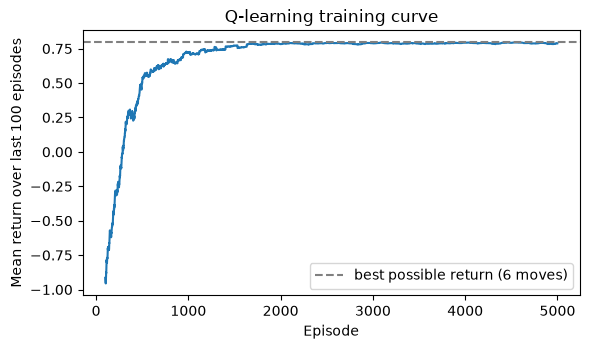
\includegraphics[width=.88\linewidth,height=5cm,keepaspectratio]{labs/visuals/06-notebook-reference.png}
\end{labvisual}

\textbf{What it means.} The first 100 episodes average a return of $-0.914$, and the last 100 average 0.788. That is just under the best possible 0.80, because 5\% of moves are still random.
\end{labanswer}

\begin{labquestion}{5}{Evaluate the greedy policy}
Training returns mix learning with random moves, so they are not a fair measure of the policy. Evaluation switches exploration off and follows the greedy policy: in each cell, take the action with the highest Q-value.
\end{labquestion}
\begin{labanswer}
\lstinputlisting[style=utppython,firstline=79,lastline=92]{all_experiments/lab06_reinforcement_worked.py}
\begin{refoutput}
\begin{lstlisting}[style=utpterminal]
success rate: 1.0
mean return: 0.8
learned action at start: down
\end{lstlisting}
\end{refoutput}

\textbf{What it means.} The goal is reached 200 times out of 200, with the best possible return. A mean of exactly 0.8 means the agent found a six-move route and never deviates from it.
\end{labanswer}

\textbf{Connect it to the chapter.} You have now run this loop 5,000 times.
% Reused from chapters/19-reinforcement-learning.tex
\begin{labvisual}{Recall the chapter model}
\begin{labgraphic}
\begin{tikzpicture}[
  node distance=3.5cm,
  box/.style={draw=UTPBlue,fill=UTPPaleBlue,rounded corners=2mm,minimum width=3cm,minimum height=1.2cm,align=center,font=\bfseries\color{UTPNavy}},
  arr/.style={-{Stealth[length=2.4mm]},thick,draw=UTPTeal}
]
\node[box] (agent) {Agent\\chooses an action};
\node[box,right=of agent] (env) {Environment\\changes state};
\draw[arr] (agent.north east) to[bend left=18] node[above,font=\small]{action $a_t$} (env.north west);
\draw[arr] (env.south west) to[bend left=18] node[below,font=\small]{state $s_{t+1}$, reward $r_{t+1}$} (agent.south east);
\end{tikzpicture}
\end{labgraphic}\end{labvisual}


\labpart{Part B --- The Q-table is the model: save it and read the policy}

\begin{labquestion}{6}{Save the table and read the policy}
Everything the agent learned is in the Q-table, so saving it is saving the model. Anyone with the file can act without retraining: in each cell, pick the action with the largest value.
\end{labquestion}
\begin{labanswer}
\lstinputlisting[style=utppython,firstline=94,lastline=103]{all_experiments/lab06_reinforcement_worked.py}
\begin{refoutput}
\begin{lstlisting}[style=utpterminal]
[['down' 'down' 'down' 'left']
 ['down' 'down' 'down' 'TRAP']
 ['right' 'down' 'down' 'down']
 ['right' 'right' 'right' 'GOAL']]
\end{lstlisting}
\end{refoutput}

\textbf{What it means.} From the start the route is down, down, right, down, right, right: six moves. A shortest route is not unique on a grid, so a different seed may pick another of the same length. The file is 640 bytes.
\end{labanswer}

\begin{labquestion}{7}{Draw the policy and the values}
The policy is easier to read as arrows on the grid, drawn over a heat map of each cell's value (the best Q-value available there). Values rise towards the goal.
\end{labquestion}
\begin{labanswer}
\lstinputlisting[style=utppython,firstline=105,lastline=126]{all_experiments/lab06_reinforcement_worked.py}
\begin{refoutput}
\begin{lstlisting}[style=utpterminal]
Best value in each cell (Q.max(axis=2)):
0.593  0.666  0.743  0.666
0.666  0.743  0.824  0.000
0.743  0.824  0.910  1.000
0.824  0.910  1.000  0.000
\end{lstlisting}
\end{refoutput}

\textbf{What it means.} These equal the exact values in \figref{fig:grid-values}, computed there without any trial and error. The agent learned them from rewards alone. The cell above the trap is worth 0.666, less than its left neighbor's 0.743, because the way out from there starts by stepping back left. The goal and trap cells are zero because no action is ever taken from them.
\end{labanswer}

\labpart{Evidence}

\begin{labquestion}{8}{Save the evidence}
Write the numbers above to the results folder. These files are regenerated on every run, so do not edit them by hand.
\end{labquestion}
\begin{labanswer}
\lstinputlisting[style=utppython,firstline=128,lastline=136]{all_experiments/lab06_reinforcement_worked.py}
\begin{refoutput}
\begin{lstlisting}[style=utpterminal]
Saved: ['greedy_policy.csv', 'greedy_policy_and_state_values.png', 'metrics.csv',
 'q_learning_training_curve.png', 'training_returns.csv', 'trap_moved_to_3_1.png']
\end{lstlisting}
\end{refoutput}
\end{labanswer}

\labpart{Try it yourself}

\begin{labquestion}{9}{Try it yourself}
Change one thing: the step cost, the trap location, the exploration schedule, or the discount factor. Write down what you expect the greedy policy to do differently before retraining, then check with \texttt{plot\_policy}. Attempt it in this empty cell before reading the solution.
\end{labquestion}

\begin{labquestion}{10}{One solution}
Move the trap onto the bottom row, at (3, 1). Prediction before retraining: the learned route runs through (3, 1), straight into the new trap, so the route has to change, for the same six-move length.
\end{labquestion}
\begin{labanswer}
\lstinputlisting[style=utppython,firstline=140,lastline=172]{all_experiments/lab06_reinforcement_worked.py}
\begin{refoutput}
\begin{lstlisting}[style=utpterminal]
Greedy policy with the trap at (3, 1):
down   down   right  down
right  down   down   down
right  right  right  down
up     TRAP   right  GOAL
\end{lstlisting}
\end{refoutput}

\textbf{What it means.} The route is now down, right, down, right, right, down: still six moves, so the return is still 0.8. The cell beside the new trap, (3, 0), points up and away from it. The right-hand column, which the original policy avoided, is now safe, and its arrows point down. The agent was never told the trap had moved; it relearned from the rewards alone.
\end{labanswer}

\begin{yourturn}
Add new cells at the end of the notebook for these tasks, using \texttt{train\_q} as a starting point. Write your prediction first, then run it.
\begin{enumerate}
  \item \textbf{No step cost.} Retrain with a step cost of 0. With no charge per move, does the agent still take a short route? Why, or why not?
  \item \textbf{A high step cost.} Retrain with a step cost of $-0.5$. Does the route change? What is its return?
  \item \textbf{Never explore.} Set $\varepsilon$ to 0 from the start. Predict whether the agent finds the goal. Then explain the result, thinking about what a $-0.04$ reward does to a Q-table that starts at zero.
  \item \textbf{Always explore.} Keep $\varepsilon$ at 1 throughout, so every training move is random. Does the \emph{greedy} policy read from the table still work?
\end{enumerate}
\end{yourturn}

\begin{expectedfindings}
\begin{enumerate}
  \item It still takes six moves, with a return of 1.00. With $\gamma=0.95$ a goal reached later is worth less, so the discount alone favors the short route.
  \item Still six moves, with a return of $5\times(-0.5)+1=-1.50$. Six moves is already the minimum, and the trap costs $-1$ at once, so the costly route is still best from the start.
  \item It reaches the goal in six moves with a return of 0.80, which may surprise you. Every tried action soon has a negative Q-value while untried ones stay at 0, so the greedy agent keeps trying whatever it has not tried. Starting at zero with negative step costs is accidental optimistic initialization. The food-stall student in Chapter~\ref{ch:rl} had no such luck, because every meal there could pay.
  \item Yes: six moves and a return of 0.80. Q-learning's backup uses the \emph{best} next action, whatever the agent actually did next, so it can learn the greedy policy's values while behaving randomly. Training returns would look terrible throughout, which is another reason to evaluate separately.
\end{enumerate}
\end{expectedfindings}

\begin{troubleshoot}
\begin{description}
  \item[The route differs from the sheet] Check whether you ran cells out of order: \texttt{rng} is shared, so rerunning a cell continues the random stream. Restart and run all. Any six-move route with return 0.8 is equally correct.
  \item[Return far below 0.8 in evaluation] Check that evaluation passes \texttt{explore=False}, and that you are not evaluating a half-trained table.
  \item[Arrows look upside down] \texttt{plt.imshow} puts row 0 at the top, so $y$ grows downward on this plot, which is why the code draws $-0.3\,dy$. Keep that sign.
  \item[The trap label is in the wrong place after the Try-it] The solution restores \texttt{TRAP} at the end of its cell. If you stopped midway, reset it to \texttt{(1, 3)}.
\end{description}
\end{troubleshoot}

\begin{labchecklists}
\begin{verification}
\begin{itemize}
  \item The greedy policy reaches the goal in six moves, for a return of $0.80$, and you can read that route from the printed policy.
  \item The success rate is reported over episodes run without exploration.
  \item \texttt{models/gridworld\_q\_table.npy} is saved, and the policy is read from the reloaded table.
  \item The first row of values matches 0.593, 0.666, 0.743, 0.666, and you can explain why the last is lower than the one before it.
\end{itemize}
\end{verification}

\begin{labdeliverable}
\begin{itemize}
  \item Restart the kernel and run all cells without errors.
  \item Submit the executed notebook, including your \emph{Your turn} cells, the generated \texttt{results/lab06/} folder, and the saved Q-table.
  \item Add a short conclusion: what you changed, what you predicted, what happened, and how the training curve differs from the greedy evaluation.
\end{itemize}
\end{labdeliverable}
\end{labchecklists}

